\documentclass[submit,techreq,noauthor]{eco}	% semi style
\usepackage[dvips]{graphicx}
\usepackage{listings, jlisting} 		% for source code
\usepackage{url}
\usepackage{setspace}
\usepackage{here}
%\setstretch{1.5} % 行間を広くします(資料チェックしてもらうときはコメントを外す)

\lstset{
  basicstyle={\ttfamily},
  identifierstyle={\small},
  commentstyle={\smallitshape},
  keywordstyle={\small\bfseries},
  ndkeywordstyle={\small},
  stringstyle={\small\ttfamily},
  frame={tb},
  breaklines=true,
  columns=[l]{fullflexible},
  numbers=left,
  xrightmargin=0zw,
  xleftmargin=3zw,
  numberstyle={\scriptsize},
  stepnumber=1,
  numbersep=1zw,
  lineskip=-0.5ex
}

\begin{document}

\semino {5/5}					% 年度/回数
\date   {5/04/25/火}				% 平成/月/日/曜日
\title  {共有ライブラリを置き換えるLinuxマルウェア:Symbioteの調査}	% タイトル
\author {奥 若菜}				% 氏名


\begin{abstract}
	Linuxにおいて,プログラム実行時に共有ライブラリを動的リンクするために使用する環境変数にLD\_PRELOADがある.
  この環境変数を使用することで,悪意のある共有ライブラリをプログラムにロードし,不正なコードを実行することをDynamic Linker Hijackingという.\cite{MITRE-ATT&CK}
  2021年に発見されたSymbioteは,すべての実行中のプロセスにロードされる共有ライブラリとして動作し,
  正当なプロセスの下で自身や他のマルウェアの痕跡を隠蔽する.
  本研究では,SymbioteのようなDynamic Linker Hijackingを行うマルウェアを動的解析し,その挙動を明らかにするとともに,効果的な検知手法の発見を目指す.
\end{abstract}
\maketitle


\section{はじめに}
近年,IoTデバイスの普及や企業のクラウドシフトにより,Linuxマシン上で動作するマルウェアが増加している.\cite{TREND-MICRO}
Linuxマシンの中にはサーバとして定常稼働しており,固定のIPアドレスが割り振られているものも多く,攻撃インフラとしての利用価値が高いことから,今後もLinuxマシンを標的とするマルウェアは増加すると予想される.

2021年に発見されたSymbioteは,Linuxで一般的に見られるマルウェアとは異なる特徴を持ち,極めて検出が困難とされる.\cite{Symbiote}
Symbioteは,単独の実行可能ファイルではなく,
すべての実行中のプロセスにロードされる共有ライブラリとして動作する.
Linuxでは,環境変数 LD\_PRELOADを使用することで,プログラムによって要求される正当な共有ライブラリの代わりに,名前の一致する悪意のある共有ライブラリを呼び出すことが可能である.
このような攻撃では正当なプロセスの下で実行がマスクされるため,プロセスベースの解析は回避される可能性が高い.

本研究は,動的解析を行うことによってSymbioteの挙動を明らかすることを目指す.
また,SymbioteのようなDynamic Linker Hijackingを行うLinuxマルウェアの検知手法および対策方法を考察する.


以下,2章でSymbioteの機能を説明し,3章で検体を用いた動的解析の結果を述べ,4章でまとめる.\\


\section{Symbiote}
Symbioteが初めて検知されたのは2021年11月であり,
ラテンアメリカの金融セクターを標的とするために作成されたとされている.
Symbioteについての調査は,Intezerの研究者Joakim KennedyとBlackBerryのResearch and Intelligence Teamによって
行われ,レポートが作成されている.以下にレポートをもとにSymbioteの機能を示す.


\subsection{検知回避機能}
Symbioteは,LD\_PRELOADで指定した共有ライブラリによって,プログラムによる関数の呼び出しをフックし,
悪意のあるコードを実行することで,検知を回避する.具体的には,C言語の標準ライブラリであるlibcおよび
パケットキャプチャのためのライブラリであるlibpcapの関数をフックすることで,以下のような回避機能を実現する.
  \begin{description}
    \item [プロセスの隠蔽] \mbox{}\\
    呼び出し元のアプリが/proc以下にあるファイルまたはディレクトリにアクセス
    しようとすると,プロセス名を元に出力を消去する.
    \item [ファイルの隠蔽] \mbox{}\\
    呼び出し元のアプリが上記以外の場所にアクセスしようとすると,暗号化さ
    れたファイルリストにある名前を元に出力を消去する.
    \item [ネットワークトラヒックの隠蔽] \mbox{}
      \begin{description}
        \item[TCP:] 
        fopenとfopen64をフックし,プロセスがproc/net/tcpを開こうとすると,該当するポートをスキップして呼び出し元に返す.
        \item[UDP:] 
        libpcap関数をフックし,受信したパケットごとにドメインの文字列をチェックする.一致した場合はそのパケットをスキップして呼び出し元に返す.
        \item[パケットキャプチャの回避:] 感染マシンがeBPFを使用してパケットキャプチャを行う際に,libc
        のsetsockopt関数をフックし,提供されたeBPFコードの前に独自のバイトコードを付加することで,ポートに基づきパケットをドロップする.
      \end{description}
  \end{description}

\subsection{ルートキット機能}
Symbioteはすべての実行中のプロセスに感染した後,認証情報の収集し,攻撃者にリモートアクセスなどのルートキット機能を提供する.

認証情報の収集は,sshやscapプロセスによって呼び出されるlibcのread関数をフックすることで行われる.
収集した認証情報はファイルに書き込まれるだけでなく,
16進エンコードされ,攻撃者が運用するサーバにDNSのAレコード要求を通じて持ち出される.\\
\indent
感染したマシンへのリモートアクセスは,Pluggable Authentication
Module(PAM)機能をフックすることで提供される.アプリケーション(telnetやssh)がPAMを利用してユーザを認証する際に,攻撃者のあら
かじめ設定したものと同じ認証情報でアクセスすると,フックされた関数が成功応答を返すとともに,攻撃者もアクセスが可能になる.

\subsection{緊急アクセス機能}
Symbioteは通常のプロセスが機能しない場合に,攻撃者のC2サーバにDNSのTXTレコード要求を送信し,マシンへの緊急アクセスを
提供する.TXTレコードの形式は,\%MACHINEID\%.\%C2\_DOMAIN\%となっている.応答を取得すると,このマルウェアはコンテンツをbase64
デコードし,コンテンツが正しいed25519秘密鍵で署名されているかどうかをチェックし,
RC4でコンテンツを復号して,生成されたbashプロセスでシェルスクリプトを実行する.\\


\section{検体の動的解析}
Symbioteの検体を隔離環境で実行し,システムコールトレースとパケットキャプチャを行った.
3.1節で解析を行った検体を紹介し,3.2節で解析環境について説明する.3.3節で検体の実行結果を示し,3.4節でDNS応答を行った場合の検体の実行結果を示す.
最後に3.5節で検体についての考察を述べる.
\subsection{検体}
Intezer AnalyzeとVirusTotalを用いてSymbioteを探索したところ,表1に示す6検体が見つかった.
これらはIntezerのレポートに記載されている検体のハッシュと一致しており,更新情報もないため,現在までで見つかっている検体は,この6検体が全てである可能性が高い.

\begin{table}[H]
  \caption{Symbioteの検体一覧}
  \label{table: Artifact}
  \centering
  \begin{tabular}{|l|l|l|}
  \hline
  No. & Hash                                                                                                        & First Seen  \\ \hline
  1   & \begin{tabular}[c]{@{}l@{}}cb4bbe3af754779e673c6ae84cb38d7f\\ 2ccbc9a1d59c52abbb98451d070dba3c\end{tabular} & 19 Aug 2022 \\ \hline
  2   & \begin{tabular}[c]{@{}l@{}}a0cd554c35dee3fed3d1607dc18debd\\ 1296faaee29b5bd77ff83ab6956a6f9d6\end{tabular} & 01 Feb 2022 \\ \hline
  3   & \begin{tabular}[c]{@{}l@{}}45eacba032367db7f3b031e5d9df10b\\ 30d01664f24da6847322f6af1fd8e7f01\end{tabular} & 29 Jan 2022 \\ \hline
  4   & \begin{tabular}[c]{@{}l@{}}ec67bbdf55d3679fca72d3c814186ff4\\ 646dd779a862999c82c6faa8e6615180\end{tabular} & 26 Jan 2022 \\ \hline
  5   & \begin{tabular}[c]{@{}l@{}}f55af21f69a183fb8550ac60f392b05d\\ f14aa01d7ffe9f28bc48a118dc110b4c\end{tabular} & 19 Jan 2022 \\ \hline
  6   & \begin{tabular}[c]{@{}l@{}}121157e0fcb728eb8a23b55457e89d45\\ d76aa3b7d01d3d49105890a00662c924\end{tabular} & 27 Nov 2021 \\ \hline
  \end{tabular}
  \end{table}

\subsection{解析環境}
解析環境を構成するソフトウェアを表2に示す.
ゲストOSからホストおよびネットワークへのアクセスはできない.
また,検体の実行と解析は全てゲストOS上で行う.

\begin{table}[H]
  \caption{解析環境}
  \label{table: 解析環境}
  \centering
  \begin{tabular}{|l|l|}
  \hline
  Guest OS   & Ubuntu 22.04.2 LTS \\ \hline
  emulator   & QEMU 6.2.0         \\ \hline
  hypervisor & KVM                \\ \hline
  Host OS    & Ubuntu 22.04.2 LTS \\ \hline
  \end{tabular}
\end{table}

\subsection{検体の実行結果}
表1に示した6検体をそれぞれ実行した結果,No.3以外の検体ではSegmentation Faultが発生したため,動作が確認できたのはNo.3のみであった.
ここではNo.3の動的解析の結果について述べる.

実行を開始すると,マルウェアは/etc/resolv.confで設定されているローカルDNSサーバ(127.0.0.53)にDNSのTXTレコード要求を送信する.
ローカルDNSサーバは外部のDNSサーバへ名前解決要求を試みるが,ネットワークに接続されていないため,到達することができない.そのため図1のように”DNS: RCODE\_SERVER\_FAILURE”というエラーメッセージが出力され,タイムアウトにより実行が終了する.

\begin{figure}[H]
	\centering
  \fbox{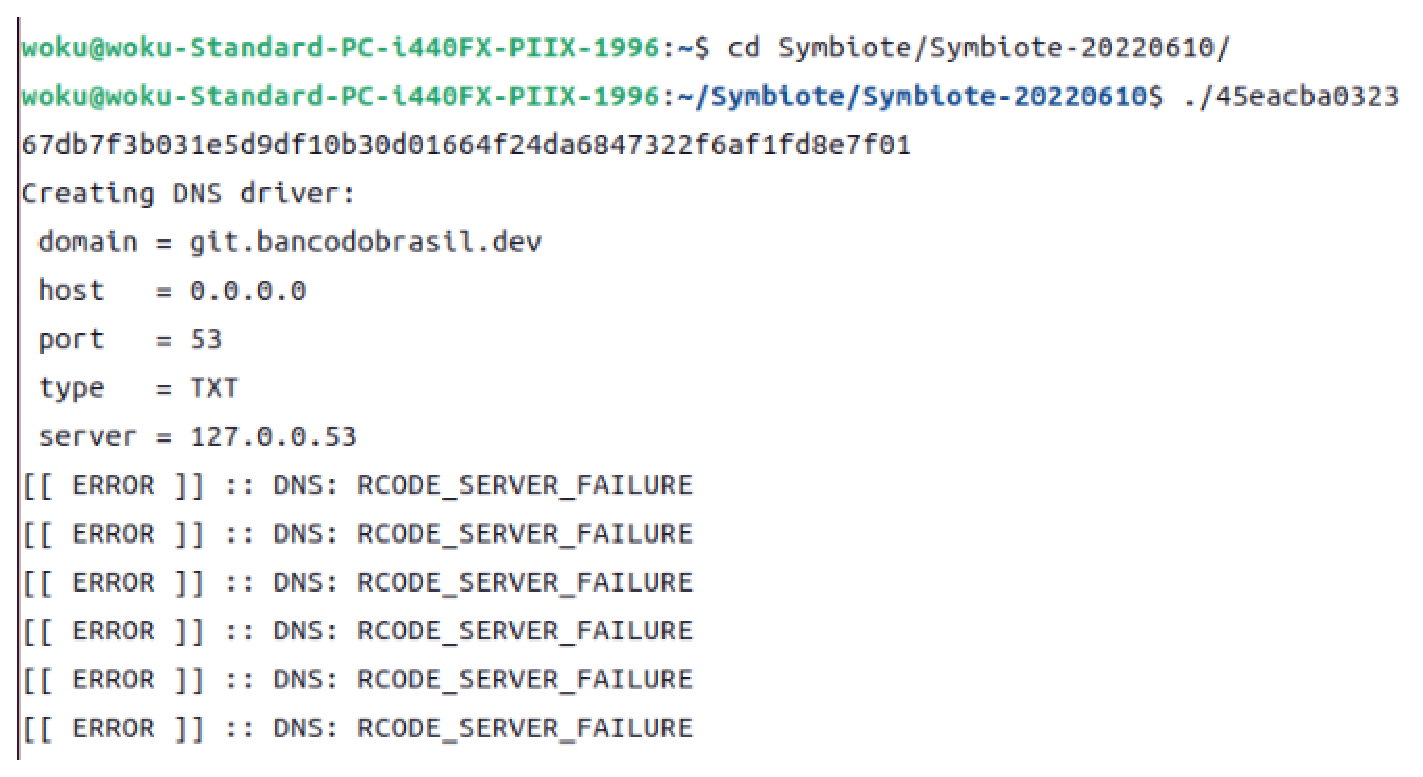
\includegraphics[width=8cm]{fig/001.eps}}
	\caption{実行結果(DNS応答なし)}
	\label{fig:001}
\end{figure}

\subsection{DNS応答を行った場合の検体の実行結果}
マルウェアを継続して動作させるためには,DNSサーバへの接続を行い,TXTレコード要求に応じる必要があると考えられる.検体が動作する環境は,ネットワークに接続していないため,外部のDNSサーバを使用することはできない.
そこで,ゲストOSのローカルポート127.0.0.1:53にDNSサーバ(ns.bancodobrasil.dev)を構築し,マルウェアへの応答を行う.

図2のパケットログより,マルウェアがDNS要求をおこなうFQDNは,リクエストごとに頭の4文字が異なることがわかる.
また,FQDNの構成は,16進エンコードされた文字列に,”git.bancodobrasil.dev”というドメインが続く形式となっている.
\begin{figure}[H]
	\centering
  \fbox{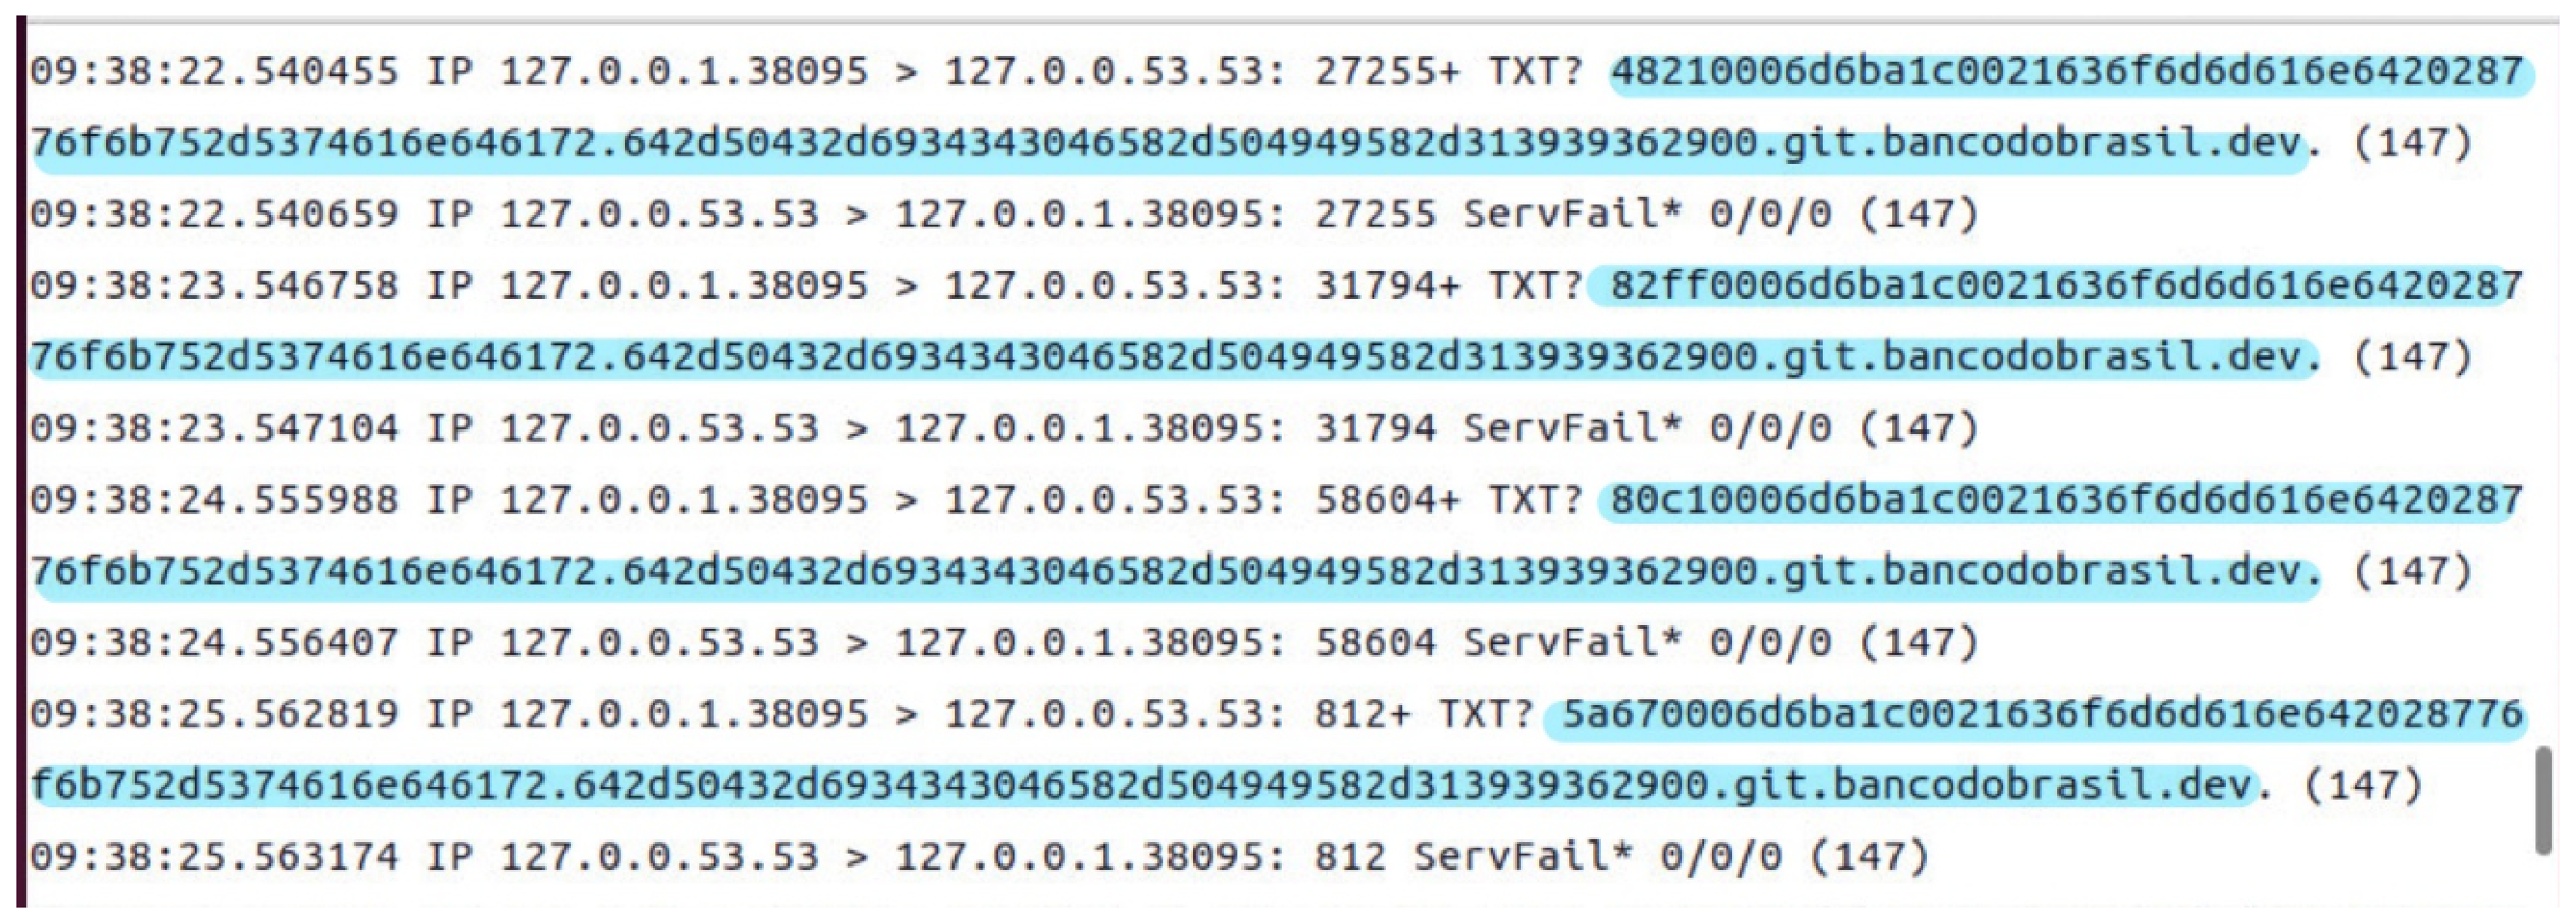
\includegraphics[width=8cm]{fig/002.eps}}
	\caption{パケットログ}
	\label{fig:packet}
\end{figure}

さらに16進でエンコードされた文字列をデコードすると,”command (woku-Standard-PC-i440FX-PIIX-1996)”という文字列が含まれることがわかる.
これは,マルウェアを実行したゲストOSのマシンIDと一致する.\\

FQDNの冒頭4文字は毎リクエストごとに異なることを踏まえ,ワイルドカードDNSレコードを使用して,DNSサーバ(ns.bancodobrasil.dev)のゾーン情報を表3のように設定した.
なお,TXTレコードの値には適当な16進数の文字列"68656c6c6f"(hello)を設定した.

\begin{table}[H]
  \centering
  \caption{DNSサーバ ゾーン情報}
  \label{table: ゾーン情報}
  \begin{tabular}{|l|l|l|l|}
  \hline
  hostname                                                                                                             & class & type & value                                                            \\ \hline
  bancodobrasil.dev.                                                                                                   & IN    & NS   & \begin{tabular}[c]{@{}l@{}}ns.bancodo\\ brasil.dev.\end{tabular} \\ \hline
  ns.bancodobrasil.dev.                                                                                                & IN    & A    & 127.0.0.1                                                        \\ \hline
  \begin{tabular}[c]{@{}l@{}}*.642d50432d6934343046\\ 582d504949582d3139393\\ 62900.git.bancodobrasil.dev\end{tabular} & IN    & TXT  & "68656c6c6f"                                                     \\ \hline
  \end{tabular}
\end{table}

  実行結果は図3のようになった.DNSのTXTレコード要求に応じることができたが,正しい値で応答していないため,"Tried to access a non-existent session(controller\_data\_incoming)"
  というエラーメッセージが出力され,タイムアウトによりマルウェアの実行が停止した.

  \begin{figure}[H]
    \centering
    \fbox{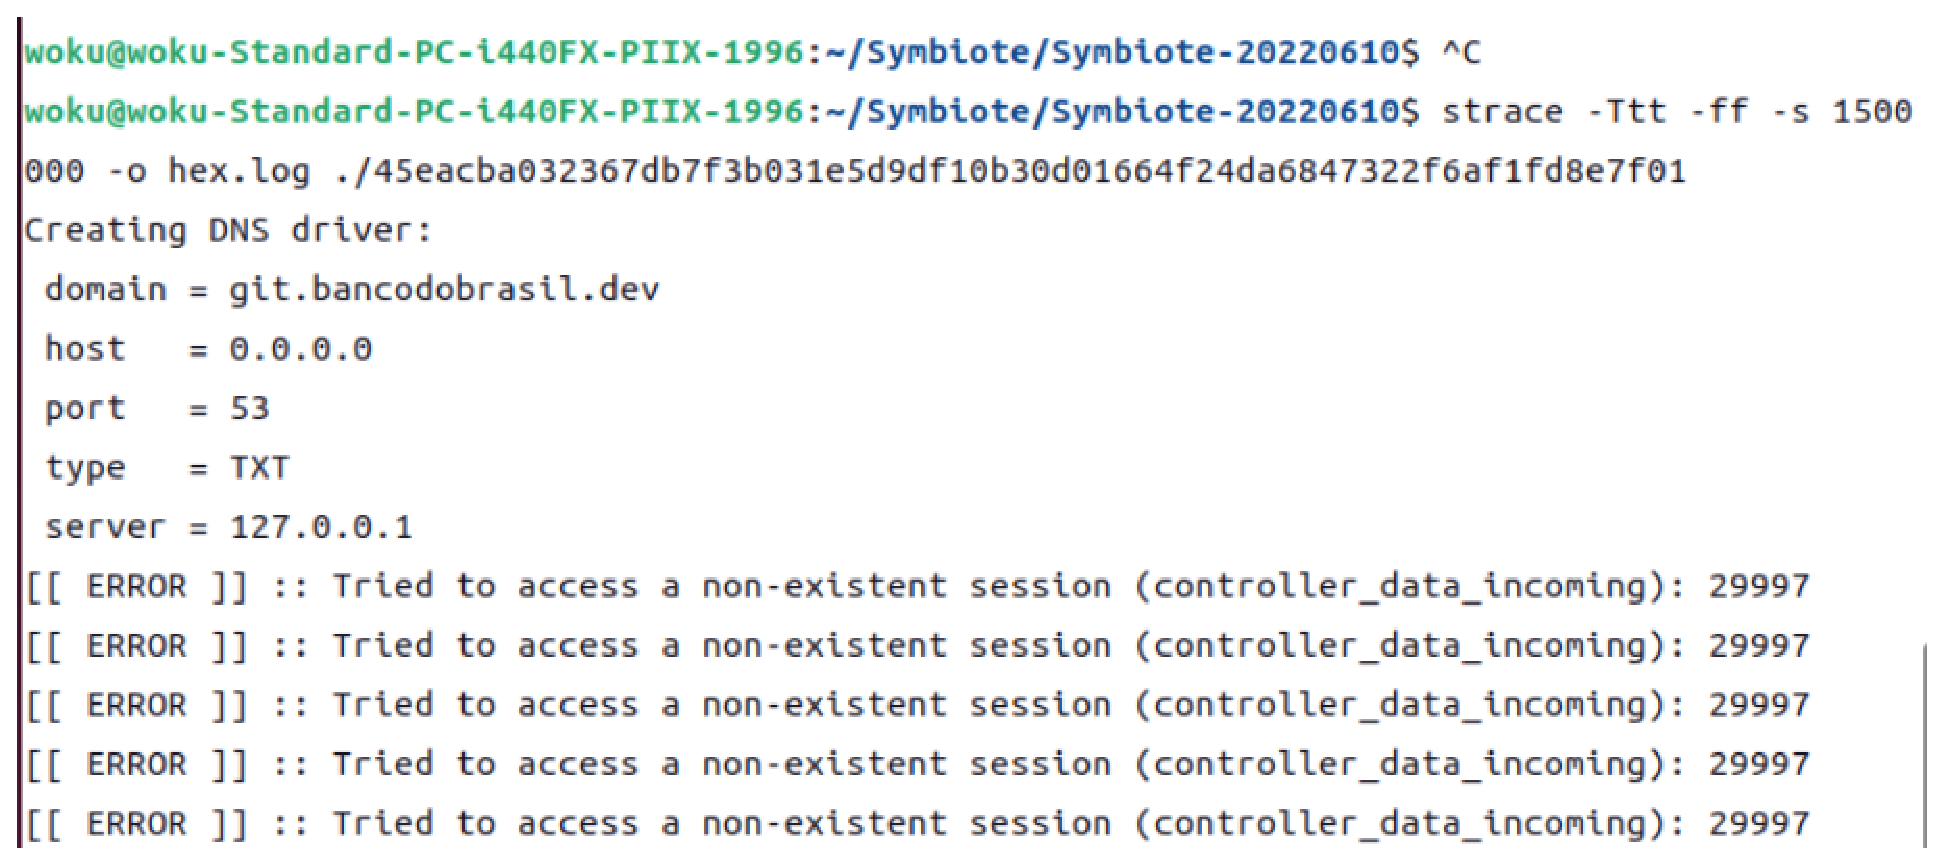
\includegraphics[width=8cm]{fig/003.eps}}
    \caption{実行結果(DNS応答あり)}
    \label{fig:003}
  \end{figure}

\subsection{考察}
No.3の検体は実行とともにDNSのTXTレコード要求を攻撃者のC2サーバに送信し,その出力やパケットが隠蔽されている様子は確認できなかった.
これらの特徴は,Symbioteの調査レポートにおける,緊急アクセス機能の特徴と一致する.よって,このマルウェアの通常プロセスは機能していない可能性が高い.
  また,DNSのTXTレコード要求に対しての応答には,攻撃者の署名が必要ということになり,これ以上の実行は困難であると考えられる.\\

\section{おわりに}
LD\_PRELOADを利用することで,共有ライブラリの置き換えを行うLinuxマルウェアである
Symbioteの調査と,その検体の動的解析を行った.結果として,現在入手している検体は
共有ライブラリの置き換えによる検知回避機能を実行する可能性が低いことがわかった.
検知が困難とされるLinuxマルウェアの効果的な解析手法を発見するために,Symbioteのような機能をもつ
他のマルウェアについても調査していく必要がある.

%bibtex
\setlength\baselineskip{12pt}
{\small
	\bibliography{references}
	\bibliographystyle{ipsjunsrt}
}


\end{document}
